\documentclass[conference]{IEEEtran}

\usepackage[pdftex]{graphicx}
% \usepackage{amsmath}
% \usepackage{afterpage}
% \usepackage{wrapfig}
% \usepackage{tabularx}
% \usepackage{subfigure}
\usepackage{caption}
\usepackage{xcolor}
% \usepackage{tabu}
% \usepackage{booktabs}
% \usepackage{multicol}
% \usepackage{hyperref}

\hyphenation{op-tical net-works semi-conduc-tor}

\usepackage[switch]{lineno}
\linenumbers
\modulolinenumbers[10]

\begin{document}

\title{DQM4HEP : A generic\\Data Quality Monitoring for High Energy Physics}

\author{

\IEEEauthorblockN{R\'emi \'Et\'e}
\IEEEauthorblockA{Univ, Lyon, Universit\'e Lyon 1, \\
CNRS/IN2P3, IPNL 4 rue E Fermi \\
69622, Villeurbanne CEDEX, France\\
Email: rete@ipnl.in2p3.fr}

\and

\IEEEauthorblockN{Antoine Pingault}
\IEEEauthorblockA{Ghent University, Department of Physics \\
and Astronomy Proeftuinstraat 86,\\
B-9000 Gent, Belgium\\
Email: antoine.pingault@ugent.be}

\and

\IEEEauthorblockN{Laurent Mirabito}
\IEEEauthorblockA{Univ, Lyon, Universit\'e Lyon 1, \\
CNRS/IN2P3, IPNL 4 rue E Fermi \\
69622, Villeurbanne CEDEX, France\\
Email: mirabito@ipnl.in2p3.fr}

}

\maketitle

\IEEEpeerreviewmaketitle

\section{Introduction}

With increasingly sophisticated devices, online data quality monitoring is of a significant importance for the detector and operation efficiency. Monitoring data is also a first step to a certification of the reliability of the recorded data for off-line physics analyses. Experiments usually develop their monitoring system on top of their event data model and file format to access and store data. This dependency has the tendency to tie the monitoring system to its dedicated experiment and leads to difficulties to adapt it to others.

With this in mind, a generic online Data Quality Monitoring (DQM) system has been developed without any assumption on the event data model (EDM) and data type to treat. A dedicated implementation, based on the LCIO~\cite{LCIO} event data model for the Linear Collider collaboration was also developed. This implementation was put to real condition testing using a combined detector setup with the CALICE~\footnote{CAlorimeter for LInear Collider Experiment} Semi-Digital Hadronic CALorimeter (SDHCAL) and Silicon Tungsten Electronic Calorimeter (SiWECal) prototypes during test beam campaigns at CERN\footnote{Conseil Européen pour la Recherche Nucléaire}.

\section{Key points and software architecture}

The framework is strongly based on a plugin system that allows some part of the software to be switched from one to another. As a consequence, the data serialization used to send data across the network is encapsulated in plugins, loaded at run-time. It is also designed to be run in separate processes linked to each other by TCP/IP or HTTP protocols using DIM\cite{DIM} and Mongoose\cite{MONGOOSE} respectively. 

\begin{figure}[htbp]
  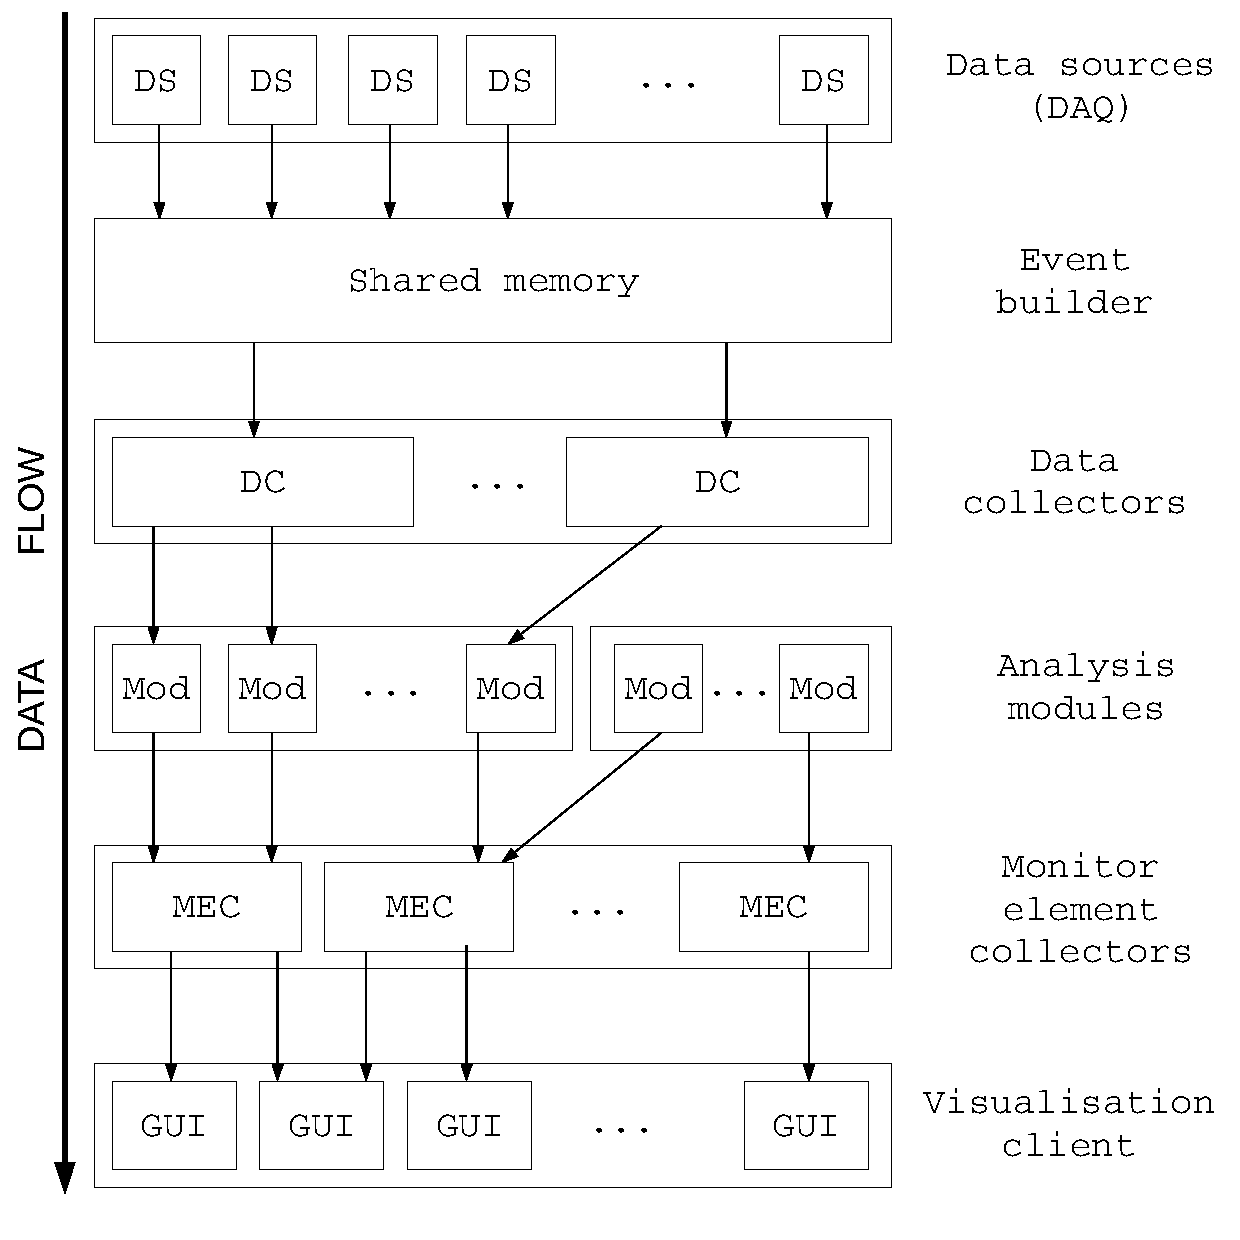
\includegraphics[width=\linewidth]{DQMWorkflow.pdf}
  \caption{\label{DQM_WORKFLOW}The monitoring framework data flow: from data sources to visualization.}
\end{figure}

Fig.~\ref{DQM_WORKFLOW} shows the monitoring framework data flow from incoming data sources to the client visualization computers. An important effort has been put on the creation of a generic interface to the data acquisition system and the development of an event builder. An independent data acquisition (DAQ) process dumps the data sources content in the shared memory (shm) until a given limit in bytes is reached (set by the DAQ). In this way, a slow data treatment by the monitoring will not affect the data taking and writing to disk. Since the data structure is setup dependent, the implementation of the event builder becomes highly specific. The event building is encapsulated in series of \textit{shm processors} that convert data sources buffers into the user data structure. The whole reconstructed event is then serialized, dispatched across the network and stored into one or multiple data collector server applications.

Client interfaces are provided to either perform manual queries of collected data or work in update mode for which the data is directly forwarded on reception. User's online data analysis are also implemented as plugins in the system and steered using configuration files, increasing the modularity of the framework. They use a data collector client interface in update mode to receive and process data.

The main aim of the online data analysis is to reduce the initial amount of data to a few monitorable quantities summarizing its quality and the status of the detection systems. Such quantities have been encapsulated in a unique interface called 'monitor element'. To evaluate the data quality, built-in template tests are provided and are frequently processed by the system. A user API is provided for the online analysis module to book \textit{monitor elements} and their quality tests which are then published across the network. They are in their turn collected by server applications and distributed to visualization clients, again, either on manual query or in update mode.

To visualize monitor elements from the collectors, a graphical user interface has been developed using the Qt\cite{QT} GUI\footnote{Graphical User Interface} toolkit. It can use multiple client interfaces to every available collectors on the network. The user can then display received \textit{monitor elements} in areas organized in tabs. Multiple configurations with different sets of monitor elements can be set-up at once. This allows for a quick overview of all the critical elements and variables needed for the good operation of the experiment.


%%%%%%%%%%%%%%%%%%%%%%%%%%%%%%%%%%%%%%%%%%%%%%%%%%%%%%%%%%%%%%%%%%%
%%%%%%%%%%%%%%%%%%%%%%%%%%%%%%%%%%%%%%%%%%%%%%%%%%%%%%%%%%%%%%%%%%%
\section{Implementation and tests}
In order to test the framework, a dedicated implementation has been developed for the CALICE collaboration and its SDHCAL and SiWEcal prototypes. 
An interface to read and write events in the LCIO format has been written using a generic data streaming toolkit named \textit{xdrstream}.

%%%%%%%%%%%%%%%%%%%%%%%%%%%%%%%%%%%%%%%%%%%%%%%%%%%%%%%%%%%%%%%%%%%

As mentioned previously, the CALICE-SDHCAL collaboration has developed tools to dump online raw data coming from the detectors to a shared memory space as data source buffers. To treat these buffers, a dedicated shm processor plugin has been implemented. It reads the data sent by the DAQ system into the shared memory, then call the online event builder (\textit{levbdim}) to reconstruct data into the lcio format. The reconstructed event is finally sent over the network to the event collector.

The LCIO EDM contains multiple data structures for different levels of reconstruction that analysis can use. To overcome this problem, data converters are provided to pass from one LCIO data structure to the other. This gives the ability to plug off-line analysis into the monitoring system, leading to a better assessment of the overall data quality.

The monitoring system can also be tested with LCIO data files as a data source. In order to keep conditions as close as possible to a real setup, it can be configured to simulate the timing structure of the raw data.

%%%%%%%%%%%%%%%%%%%%%%%%%%%%%%%%%%%%%%%%%%%%%%%%%%%%%%%%%%%%%%%%%%%
For the two weeks beam test campaign at CERN, specific analysis aimed to the monitoring of the SDHCAL and SiWEcal have also been developed. They come as independent modules to plug into the framework and can be started or stopped at any given time. This implies that even a buggy analysis that would come to crash will not interfer with the rest of the monitoring. All the modules are configurable either through xml files or command line: most of the parameters can be quickly adjusted, a few seconds prior to start the module.

Part of the monitoring includes a module to watch the slow control parameters (high and low voltages, pressure, temperature, etc.). As these information do not come from the DAQ system, it is developed as a standalone module (see right analysis module block in Fig.~\ref{DQM_WORKFLOW}).
One analysis is dedicated to the raw data study and permits the shifters to quickly discover and try to correct for noisy part of the detector. A beam study analysis is available to display metrics about the beam spill such as its length, time structure, number of acquisition cycle per spill, etc. Some \textit{monitor elements} from this module can also be used as performances indicators. One practical example would be the ratio between the number of events treated by the monitoring and the DAQ systems.

Other modules are dedicated to efficiency measurement of various parts of the detectors, particle identification or tracking. Specific information using core properties of the detectors are also recorded like the deposited energy (SiWEcal) or number of hits for each threshold (SDHCAL). Finally event display modules are also present to visualise particle interactions inside the detectors.

The Marlin\cite{MARLIN} framework being widely used within the Linear Collider Collaboration for data analysis, an interface is under development and will permit users to directly plug their analysis as it is into the monitoring.

For the test beam campaign at CERN the framework has been successfully deployed across multiple computers, each one running a set of collectors (\textit{monitor element} and event) and analysis modules. Several monitoring GUIs were running on these computers and personal shifters equipment.


\section{Conclusion}
In light of the critical importance of a mean to quickly detect problems and ensure a good data quality, a new generic framework for Data Quality Monitoring systems has been created.

Contrary to most systems available for High Energy Physics up to now, it is not tied to a given experiment set-up. All the tools needed to develop a specific implementation depending on specificities of the experiment, such as DAQ interface, data format and detector analysis, are provided within the framework.
To put to test this system, a dedicated implementation has been developed in parallel for the CALICE SDHCAL and SiWEcal collaborations. The whole system has been successfully used to monitor both prototypes during a two weeks beam test campaign at CERN. The results are satisfactory and the framework is now in its final stage. Other collaborations within the LCC already manifested their interest to use this system for their technological prototypes.

\begin{thebibliography}{1}
  
\bibitem{QT}
Qt Company, \emph{\tt http://www.qt.io}, v4.7, 2016.

\bibitem{DIM}
C. Gaspar et al., \emph{DIM”, International Conference on Computing in High Energy and Nuclear Physics} (Padova,  Italy,
1-11 February 2000)

\bibitem{MONGOOSE}
Michael J Hammel. \emph{Mongoose: an embeddable web server in C}, Linux Journal, 2010(192):2, 2010.

\bibitem{ROOT}
I. Antcheva \textit{et al.}, Comput. Phys. Commun. \textbf{182}, 1384 (2011)

\bibitem{MARLIN}
F. Gaede, {\it Marlin and LCCD: Software tools for the ILC}, {\tt Nucl.Instrum.Meth. A559 (2006) 177-180}

\bibitem{LCIO}
Frank Gaede, \emph{\tt lcio.desy.de}, 2016.

\end{thebibliography}
  
\end{document}
